\chapter{Datasets}
In this chapter, a description of the datasets used in the experiments is provided. Four public datasets, one private dataset, and one additional dataset constructed by merging several public datasets were used in this thesis. In the first section of this chapter, the datasets are presented individually. This includes information about their size, content (whether they contain only phishing URLs or also other types of malicious URLs), and how the data was collected. The next section presents the exploratory data analysis performed on the datasets, highlighting both the methods used and the key insights obtained.

\section{Individual Dataset Descriptions}
\label{sec:dataset_descriptions}

\subsection{GramBeddings}
The dataset consists of approximately 800,000 URLs, evenly split between phishing and benign URLs. It was developed as a part of the paper~\cite{GramBeddings}.

The data has been collected over a long-term period (May 2019 -- June 2021), with weekly sampling intervals. After all data was collected, the authors post-processed the URLs to filter them with almost identical domain information.

The phishing URLs were collected from PhishTank~\cite{PhishTank} and OpenPhish~\cite{OpenPhish}. These online services collect, verify, and provide phishing URL lists. Anyone can use their website or API to check whether a given URL is classified as phishing. PhishTank, operated by Cisco Talos, allows users to report and validate phishing sites, maintaining a community-driven blocklist. Since data is labelled by humans, it achieves high accuracy but takes longer to classify phishing URLs. OpenPhish is an automated service that continuously crawls and analyzes phishing URLs using machine learning methods, offering free and commercial threat feeds.

Benign URLs were collected using a custom web crawler. In the beginning, it downloaded the content of the 20 most popular websites in each country. Then, all links from these websites are extracted and filtered to remove duplicates and similar URLs. Now, the content of websites behind these URLs is downloaded and processed in the same way. This process is repeated until the desired number of benign URLs is reached, which in this case was 2 million. A subset of 400,000 URLs was randomly selected to match the number of phishing URLs. This method should produce a diverse set of benign URLs as it is expected that popular websites are not phishing sites themselves, nor do they contain links to phishing sites.

\subsection{Mendeley}
The Mendeley dataset~\cite{Singh2020Mendeley} comprises 1,561,934 URLs, exhibiting a substantial class imbalance with 1,526,619 benign URLs and 35,315 malicious URLs, leading to a 1:43 skew in favour of benign URLs. Unlike the GramBeddings dataset, this one marks every category of harmful URLs described in previous sections as malicious, not just phishing. The original dataset contains more information than just URL and label, but for the purposes of this study, only these two fields were used.

The dataset was constructed using a specialized crawler designed to crawl more malicious URLs than traditional crawlers. The labels are then classified as either benign or malicious using Google Safe Browsing API~\cite{GoogleSafeBrowsing}, which is a similar service as PhishTank and OpenPhish mentioned earlier. The data was collected for an unknown period of time up to May 2020.

The Mendeley dataset is closer to real-world web distributions, where malicious URLs are significantly outnumbered by benign ones. This imbalance presents challenges in training machine learning models, as classifiers may become biased towards the majority class. On the other hand, it makes it a good benchmark for evaluating model performance in realistic scenarios. However, the number of malicious URLs is rather small compared to all other datasets, especially the private dataset~\ref{sec:private_dataset}, which is imbalanced too but has significantly more malicious samples (283,616).

\subsection{Kaggle Multiple}
This dataset~\cite{SiddharthaMaliciousURLs} is used for a multi-class classification and consists of 651,191 URLs categorized into four classes:

\begin{itemize}
    \item 342,651 benign (safe) URLs —- Primarily collected from the ISCX-URL-2016 dataset~\cite{ISCX-URL-2016}. It was collected in 2016.
    \item 18,857 malware URLs -- Sourced from a specialized malware dataset and the ISCX-URL-2016 dataset.
    \item 76,252 defacement URLs —- Extracted from the ISCX-URL-2016 dataset. The defacement attack \cite{wikipedia2024defacement} involves altering the content of a legitimate website to display unauthorized or malicious content. This is often done through SQL injection or other vulnerabilities in the web application. Since the website is legitimate and only the content is altered, the URL itself does not have enough information to detect this type of attack. Therefore, all of the URLs with this class are removed from the dataset.
    \item 75,135 phishing URLs —- Gathered from multiple sources, including PhishTank and PhishStorm~\cite{Marchal2014PhishStorm}. PhishStorm contains data up to 2014. The collection period for the PhishTank data is unspecified.
\end{itemize}

This dataset is used in Section~\ref{sec:multi_class_experiment}, which checks whether the URL-string-based models can be used for multi-class classification after domain-aware folding introduced in Section~\ref{sec:train_test_split} is applied.

\subsection{Kaggle binary}
The Kaggle binary dataset~\cite{KaggleBinaryDataset} consists of 632,503 URLs, evenly distributed between 316,252 benign URLs and 316,251 malicious URLs. Because of the way the dataset was constructed, it can be assumed that URLs labelled as malicious are pointing to either phishing, malware or defacement. The dataset was constructed by combining and preprocessing data from two separate publicly available Kaggle datasets:
\begin{itemize}
    \item First dataset -- Contains 450,176 URLs, with 77\% benign and 23\% malicious URLs. Malicious data were collected using PhishTank and an unknown number of other services. They may or may not include non-phishing malicious URLs. The last update for this dataset was in 2019.
    \item The second dataset -- Kaggle Multiple datasets described earlier. Initially, all URLs labelled as phishing, defacement, and malware were added to this dataset under the "malicious" label. All URLs labelled as defacement in the previous dataset must also be manually removed from this one to ensure consistency with the chosen detection approach.
\end{itemize}

\subsection{Private Dataset}
\label{sec:private_dataset}
This dataset was provided by the supervisor and consists of real-world data from the customers that want to check, whether URL is malicious or not. It was collected in August 2024 by Cisco Talos. It consists of 2,836,160 URLs, with 2,552,544 labeled as benign (90.0\%) and 283,616 labeled as malicious (10.0\%). The dataset was created by down-sampling benign URLs from an even more imbalanced distribution to make training focus more on the malicious samples.

Unlike the public datasets, this dataset has undergone pre-filtering, meaning many obviously benign or trivially malicious URLs were excluded before labeling. As a result, the classification on this dataset is more difficult, since the remaining examples tend to be more ambiguous or sophisticated.

Due to confidentiality restrictions, the private dataset cannot be included in this thesis. However, experimental evaluations performed on this dataset are provided and discussed in later chapters. This offers insights into how the model performs on real-world data and illustrates how well evaluation results obtained on public datasets translate to real-world scenarios.

\subsection{Joined Dataset}
A new dataset was created by merging the GramBeddings, Kaggle Binary, and Mendeley datasets. The goal was to expose the model to a wider variety of URL patterns and malicious behaviors while addressing the shortcomings of individual datasets -- GramBeddings and Kaggle Binary are balanced but small, while Mendeley lacks sufficient malicious samples.

Although combining datasets introduces variations in data distributions, this approach aligns with the original public datasets, which were themselves assembled from multiple other datasets and sources.

After preprocessing, the final dataset contains 2,862,060 URLs: 2,194,899 labeled as benign (76.69\%) and 667,161 labeled as malicious (23.31\%). A total of 8,296 URLs (approximately 0.29\%) were dropped during preprocessing due to deduplication and filtering.

\section{Preprocessing}
This section describes the key preprocessing steps applied to the raw public datasets to prepare them for training and evaluation. The private dataset was already preprocessed prior to use and, therefore, required no additional modifications. Everything described here is present in \texttt{data\_preprocessing.ipynb} notebook.

\subsection{Conflicts and Duplicates}
A label conflict arises when the same URL is duplicated and is assigned different labels, either within a single dataset or across multiple datasets. No such conflicts were detected in Kaggle Binary, Kaggle Multiple, or GramBeddings. However, some were found in the Mendeley dataset, likely due to changes in the Google Safe Browsing API responses, initially misclassifying certain URLs and later returning corrected labels upon re-evaluation.

Since no dataset provides timestamps, it is impossible to tell which label is more recent or accurate. All conflicting entries were therefore removed globally. In total, 215 records (105 unique URLs) were deleted -- mostly from Mendeley (195), with smaller contributions from Kaggle Binary (12), Kaggle Multiple (5), and GramBeddings (3).

Aside from these conflicts, there are no duplicates within dataset in GramBeddings, Kaggle Binary, or Kaggle Multiple. However, for Mendeley, 3.05\% of all records are duplications. All of them are removed from the dataset.

When joining the GramBeddings, Kaggle Binary, and Mendeley datasets to create the Joined dataset, 8,296 URLs (0.28\%) were found to be shared between multiple datasets. No URL appears in all three of them. Additionally, only two URLs are shared between the private dataset and any of the public datasets.

\subsection{Train-Test Split}
\label{sec:train_test_split}
The majority of papers in the related work use a simple random split strategy, such as an 80/20 or 90/10 train-test split. However, this leads to unrealistic evaluations. The vast majority of URLs with the same second-level domain in these datasets are either entirely benign or entirely malicious, allowing models to achieve high predictive performance by memorizing domain labels rather than learning generalizable patterns.

Table~\ref{tab:sld_label_distribution} confirms this issue, showing that in nearly all datasets, over 98\% of second-level domains are associated exclusively with either benign or malicious URLs.

\begin{table}[H]
    \centering
    \renewcommand{\arraystretch}{1.2}
    \resizebox{\textwidth}{!}{
        \begin{tabular}{lccc}
            \toprule
            \textbf{Dataset} & \textbf{100\% Malicious} & \textbf{100\% Benign} & \textbf{Mixed Labels} \\
            \midrule
            GramBeddings     & 29.34\%                  & 70.32\%               & 0.34\%                \\
            Kaggle Binary    & 53.63\%                  & 44.77\%               & 1.60\%                \\
            Kaggle Multiple  & 31.12\%                  & 66.03\%               & 2.85\%                \\
            Mendeley         & 2.36\%                   & 97.50\%               & 0.13\%                \\
            Private          & 4.71\%                   & 94.93\%               & 0.36\%                \\
            Joined           & 15.31\%                  & 82.94\%               & 1.75\%                \\
            \bottomrule
        \end{tabular}
    }
    \caption{Distribution of second-level domains by label purity. "Mixed Labels" indicates domains that contain both benign and malicious URLs. For Kaggle Multiple, everything non-benign is considered malicious.}
    \label{tab:sld_label_distribution}
\end{table}

To enable more reliable evaluation, in this work, the dataset is split so that no second-level domain appears in both the train and test set. More generally, the data is partitioned into N folds, ensuring that all URLs sharing the same domain are assigned to the same fold. This thesis uses 5-fold splitting for public datasets. Four folds were used for the training set and one for the test set. The private dataset is split into 10 folds, and 1 of them is used as a test set. During the experimentation, the test set is kept separately and is never trained on.

Figure~\ref{fig:folds} illustrates the difference between standard random splitting and domain-aware folding. It should be noted, however, that this method does not improve training quality itself. It just provides better insights into real generalization capabilities. The newly proposed method to force the model to generalize is then discussed in Section~\ref{sec:domain_masking}.

\begin{figure}[H]
    \centering
    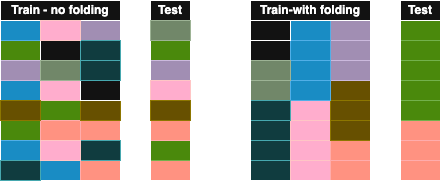
\includegraphics[width=0.8\textwidth]{images/folds.png}
    \caption{Comparison of random train-test splitting and second-level domain (SLD)-based folding. In the diagram, each column represents a fold within the train or test set, each block corresponds to a URL, and each colour represents a distinct second-level domain. It is important that in domain-based folding, the same colour is not in both train and test sets}
    \label{fig:folds}
\end{figure}

When constructing the folds, two constraints should be balanced:
\begin{itemize}
    \item All folds should be approximately equal in size to maintain consistent training and testing set sizes
    \item Each fold should preserve the original class distribution of the dataset (e.g., a 9:1 benign-to-malicious ratio should be maintained within each fold)
\end{itemize}
Table~\ref{tab:sld_folding_statistics} shows an example of how the dataset is distributed when using folding on the Joined dataset.

After initial construction, the folds are sorted by the Gini index of domain frequency, an example of which can be seen in Table~\ref{tab:sld_folding_statistics}. The fold with the lowest Gini index is selected as the test set. This ensures that the test set is as uniform as possible with respect to counts of URLs for SLDs. This helps to avoid scenarios where, for example, a single SLD makes up 12\% of the test set and offers little to helpful none indicators of maliciousness beyond the domain name itself. The model would have no way of detecting these URLs and would be unjustly penalized in such cases, even if it generalizes well. The fact that folds are ordered is also helpful for hyper-parameter tuning because the evaluation set is just picked to be the next fold with the lowest Gini index.

\begin{table}[H]
    \centering
    \renewcommand{\arraystretch}{1.2}
    \resizebox{\textwidth}{!}{
        \begin{tabular}{lllllllllll}
            \toprule
            \textbf{Fold} & \textbf{URLs} & \textbf{SLDs} & \textbf{Benign} & \textbf{Benign \%} & \textbf{Malicious} & \textbf{Malicious \%} & \textbf{Top 1 SLD}    & \textbf{Top 2 SLD} & \textbf{Top 3 SLD}  \\
            \midrule
            0             & 572{,}662     & 245{,}422     & 444{,}298       & 77.58              & 128{,}364          & 22.42                 & geocities (9.3\%)     & appspot (1.8\%)    & alibaba (1.5\%)     \\
            1             & 572{,}351     & 255{,}202     & 449{,}272       & 78.50              & 123{,}079          & 21.50                 & tripod (4.1\%)        & wikipedia (3.1\%)  & blogspot (2.7\%)    \\
            2             & 572{,}349     & 264{,}155     & 444{,}623       & 77.68              & 127{,}726          & 22.32                 & angelfire (3.9\%)     & yahoo (2.5\%)      & imdb (2.3\%)        \\
            3             & 572{,}349     & 274{,}267     & 414{,}583       & 72.44              & 157{,}766          & 27.56                 & 000webhostapp (3.7\%) & ietf (1.1\%)       & sourceforge (0.8\%) \\
            4             & 572{,}349     & 281{,}081     & 442{,}123       & 77.25              & 130{,}226          & 22.75                 & newadvent (2.0\%)     & google (0.6\%)     & about (0.6\%)       \\
            \bottomrule
        \end{tabular}
    }
    \caption{Summary statistics for the 5-fold split of the Joined dataset. Each row corresponds to a fold, showing the number of URLs, number of unique SLDs, class distribution (benign vs. malicious), and the top three most frequent SLDs with their relative frequencies. Fold 4 is used as a test set.}
    \label{tab:sld_folding_statistics}
\end{table}

The effect of domain-aware folding on evaluation performance is shown in Table~\ref{tab:folding_comparison}. Without folding, models appear to perform substantially better in all important metrics. For more information about them, see Section~\ref{sec:metrics}. This is particularly evident in the case of BERT-Tiny~\cite{turc2019} on the private dataset.

A similar case of overestimated performance for smaller models appears when comparing BERT-Small on the GramBeddings dataset in this thesis to the BERT-base results reported in~\cite{domurlbert}. In their work, BERT-base achieved a class 1 F1 score of 0.983 on GramBeddings—the same score obtained here by BERT-Small when domain-aware folding was not applied. This illustrates why results from related work that do not use folding-based evaluation should be interpreted with caution, as they may give an overly optimistic impression of model generalization.

\begin{table}[H]
    \centering
    \renewcommand{\arraystretch}{1.2}
    \resizebox{\textwidth}{!}{
        \begin{tabular}{lllll}
            \toprule
            \textbf{Model} & \textbf{Dataset}                      & \textbf{F1$_1$} & \textbf{Rec$_1$} & \textbf{Prec$_1$} \\
            \midrule
            BERT-Small     & GramBeddings \textbf{Without Folding} & 0.9834          & 0.9820           & 0.9848            \\
            BERT-Small     & GramBeddings With Folding             & 0.9662          & 0.9798           & 0.9530            \\
            \midrule
            BERT-Tiny      & private \textbf{Without Folding}      & 0.935           & 0.9071           & 0.9649            \\
            BERT-Tiny      & private With Folding                  & 0.7565          & 0.6874           & 0.8411            \\
            \bottomrule
        \end{tabular}
    }
    \caption{Comparison of performance with and without SLD-based folding using BERT models with baseline parameters shown in Section~\ref{sec:BERT-Tiny-finetune}. Each model in a pair has the same parameters.}
    \label{tab:folding_comparison}
\end{table}

\section{Exploratory analysis}
This section is based on the \texttt{data\_exploration.ipynb} notebook. The most noteworthy findings were selected and described here.

\subsection{Hostname}

One part of the hostname is TLD. Malicious URLs exhibit distinct TLD distributions compared to benign URLs. Table~\ref{tab:benign_malicious_tld} highlights the differences.

\begin{table}[H]
    \centering
    \renewcommand{\arraystretch}{1.2}
    \resizebox{\textwidth}{!}{
        \begin{tabular}{llllllll}
            \toprule
            \textbf{Dataset} & \textbf{.com (B/M)} & \textbf{.net (B/M)} & \textbf{.org (B/M)} & \textbf{ccTLD (B/M)} & \textbf{Other (B/M)} \\
            \midrule
            GramBeddings     & 49.80\% / 52.52\%   & 3.46\% / 3.77\%     & 8.09\% / 2.97\%     & 26.47\% / 20.39\%    & 11.19\% / 20.34\%    \\
            Kaggle Binary    & 77.06\% / 46.54\%   & 3.32\% / 4.80\%     & 9.68\% / 5.79\%     & 3.94\% / 20.05\%     & 4.04\% / 21.50\%     \\
            Kaggle Multiple  & 72.25\% / 47.12\%   & 4.44\% / 4.86\%     & 8.75\% / 8.22\%     & 7.48\% / 14.70\%     & 5.44\% / 22.40\%     \\
            Mendeley         & 60.98\% / 71.94\%   & 4.58\% / 6.58\%     & 12.33\% / 2.65\%    & 6.22\% / 13.75\%     & 10.60\% / 5.05\%     \\
            Joined           & 61.26\% / 51.33\%   & 4.20\% / 4.28\%     & 11.18\% / 3.97\%    & 9.58\% / 19.94\%     & 9.77\% / 20.01\%     \\
            Private          & 48.48\% / 46.91\%   & 5.73\% / 4.61\%     & 3.23\% / 0.96\%     & 16.52\% / 19.94\%    & 26.02\% / 27.57\%    \\
            \bottomrule
        \end{tabular}
    }
    \caption{Comparison of TLD distributions between benign (B) and malicious (M) URLs. The values were obtained by splitting each dataset into benign and malicious subsets and calculating the percentage of URLs in each subset that contain a given TLD type. CcTLD refers to country-code top-level domains such as \textit{.uk}, \textit{.de}, or \textit{.fr}. The "Other" category includes all remaining TLDs not covered by the standard groups, such as \textit{.xyz}, \textit{.biz}, and .info, as well as URLs that use IP addresses instead of domain names or URLs that contain malformed TLDs.}
    \label{tab:benign_malicious_tld}
\end{table}

Another part of the hostname is SLD. When looking at the datasets, certain second-level domains appear more frequently than others. The information about the content behind the domain is unknown to the model, however, it is useful for the reader to gain insight into what kind of data there are in the dataset.

Many benign URLs belong to widely used platforms like Wikipedia, YouTube, and Facebook. In contrast, malicious URLs frequently originate from free hosting services, dynamic DNS providers, and public cloud platforms.

Malicious SLDs often fall into the following categories:
\begin{itemize}
    \item Free Hosting services: (\textit{000webhostapp}, \textit{netlify}, \textit{appspot}, \textit{pastehtml}) allow easy, anonymous site creation, making them ideal for phishing and malware. Almost all of the URLs containing these SLDs are labelled as malicious.
    \item Free cloud storage services: (\textit{googleapis}, \textit{microsoft}, \textit{google}, \textit{ibm}, \textit{sharepoint}). These can freely host malicious content, making them popular among attackers. It provides valuable insight that just because a URL contains a common serious domain like \textit{google} does not mean it is benign.
    \item Less known SLDs usually have a higher probability of containing malicious intent as they are not yet verified.
\end{itemize}

\subsection{Statistical Analysis of URL Characteristics}
\label{sec:statistical_analysis_url}

To better understand URL structure across datasets, 43 manually engineered features were extracted from the dataset. They were chosen based on the findings from Section~\ref{sec:man_feat_eng}. The code for the features has been from a large majority generated by ChatGPT O1~\cite{openai2025features}. Table~\ref{tab:selected_url_features} shows a subset that highlights key differences by dataset and label. These features are primarily included to give the reader a clearer sense of how the data is distributed. Full statistics are available in the exploration notebook.

Some interesting findings from it are:
\begin{itemize}
    \item Because of pre-filtering for private datasets, many superficial heuristics have reversed values: benign URLs are longer, contain more digits, and have more non-alphanumeric characters than malicious ones.
    \item In datasets like GramBeddings, Joined dataset, and Kaggle Binary, malicious URLs are systematically longer and more complex than benign ones.
    \item The Kaggle Multiple dataset shows that the malware class uses IP-based domains at a much higher rate than the phishing or benign classes, indicating that different attack types exploit different structural patterns.
    \item In public datasets, the presence of an IP address in the URL is a strong indicator of maliciousness, largely because crawlers rarely encounter benign IP-based URLs in the wild. These datasets are biased toward visible web content, where legitimate services typically use domain names. In contrast, the private dataset includes traffic, where IP addresses are also used in benign contexts.
\end{itemize}

\begin{table}[H]
    \centering
    \renewcommand{\arraystretch}{1.2}
    \resizebox{\textwidth}{!}{
        \begin{tabular}{lllllll}
            \toprule
            \textbf{Dataset} & \textbf{Label} & \textbf{URL Length} & \textbf{Num Digits} & \textbf{Non-Alnum} & \textbf{IP in SLD (\%)} & \textbf{kw\_login (\%)} \\
            \midrule
            Private          & Benign         & 186.47              & 38.72               & 17.60              & 6.10                    & 1.75                    \\
            Private          & Malicious      & 121.64              & 18.90               & 12.82              & 5.84                    & 5.43                    \\
            GramBeddings     & Benign         & 46.43               & 1.82                & 8.68               & 0.05                    & 0.54                    \\
            GramBeddings     & Malicious      & 86.21               & 14.98               & 11.83              & 3.36                    & 0.54                    \\
            Joined           & Benign         & 41.01               & 1.33                & 7.95               & 0.04                    & 0.06                    \\
            Joined           & Malicious      & 73.54               & 11.06               & 10.72              & 4.70                    & 0.15                    \\
            Kaggle Binary    & Benign         & 58.30               & 3.26                & 10.46              & 0.09                    & 0.03                    \\
            Kaggle Binary    & Malicious      & 57.80               & 6.01                & 9.33               & 7.52                    & 0.03                    \\
            Kaggle Multiple  & Benign         & 57.69               & 5.60                & 8.51               & 0.14                    & 0.15                    \\
            Kaggle Multiple  & Malware        & 46.55               & 11.07               & 9.40               & 49.90                   & 0.28                    \\
            Kaggle Multiple  & Phishing       & 45.98               & 3.69                & 6.78               & 0.56                    & 0.45                    \\
            Mendeley         & Benign         & 35.84               & 0.79                & 7.22               & 0.03                    & 0.02                    \\
            Mendeley         & Malicious      & 37.20               & 0.29                & 7.68               & 0.00                    & 0.01                    \\
            \bottomrule
        \end{tabular}
    }
    \caption{Key URL statistics by dataset and label. Num Digits counts numeric characters; Non-Alnum counts non-alphanumeric characters; IP in SLD (\%) is the percentage of URLs whose second-level domain is an IP address; kw\_login (\%) is the percentage containing the substring login.}
    \label{tab:selected_url_features}
\end{table}

\subsection{URL Length}
\label{sec:url_length}

The URL length, examined in Table~\ref{tab:url_length_summary}, plays an important role in inference speed, as longer URLs increase the processing time for all model types. In models that rely on batched input, such as BERT, shorter URLs are padded to match the length of the longest sequence in the batch (or the predefined maximum length, whichever is smaller). This padding causes even short URLs to be processed as if they were long, resulting in unnecessary computational overhead. Consequently, measurements on datasets with lower variance in URL length tend to give higher inference speed results. This behaviour is clearly observed on the Mendeley dataset, as discussed in Section~\ref{sec:baselines}. The exact opposite case of that is the private dataset.

\begin{table}[H]
    \centering
    \renewcommand{\arraystretch}{1.2}
    \begin{tabular}{lllll}
        \toprule
        \textbf{Dataset} & \textbf{Mean} & \textbf{Median} & \textbf{Std. Dev.} & \textbf{Max} \\
        \midrule
        GramBeddings     & 66.322        & 49.000          & 59.071             & 7833         \\
        Kaggle Binary    & 58.082        & 49.000          & 39.542             & 2314         \\
        Kaggle Multiple  & 55.191        & 43.000          & 43.944             & 2175         \\
        Mendeley         & 35.872        & 32.000          & 14.440             & 721          \\
        Joined           & 48.593        & 38.000          & 39.577             & 7833         \\
        Private          & 179.990       & 107.000         & 291.134            & 110511       \\
        \bottomrule
    \end{tabular}
    \caption{Summary statistics for raw URL length in each dataset.}
    \label{tab:url_length_summary}
\end{table}